\section{Experimentos}


	Como lo han mostrado \cite{Hess1975}, \cite{Azuma} y \cite{Lorenz}, hasta ahora, la trayectoria de vuelo real de un boomerang se ha comparado con la obtenida en simulación a traves de videos o imagenes y dispositivos emisores de luz embarcados en este. Sin embargo esto ha sido con la intención de obtener una comparativa cualitativa, no cuantitativa.

	En este caso se ha optado por la instrumentación de un boomerang debido a lo interesante de la idea de obtener una trayectoria de vuelo cuantificada, además de que con esto será posible, posteriormente, no solo comparar los resultados reales con los obtenidos en simulación, sino buscar la parametrización del modelo.

	\subsection{Obtención y procesamiento de datos}

	Se describirán brevemente los dispositivos que conforman la unidad registradora de datos y se dará una breve explicación de las herramientas que se utilizaron para procesar estos últimos.

	\subsubsection{Dispositivos utilizados}

	\subsubsection{Unidad de medición inercial, 9DOF Razor IMU}

	Definición. Una unidad de medición inercial o IMU (del inglés Inertial Measuremente Unit) es un dispositivo electrónico que mide e informa acerca de velocidad, orientación y fuerzas gravitacionales de un aparato, usando una combinación de acelerómetros y giroscópios.

	La unidad de medición inercial 9DOF Razor IMU de Sparkfun incorpora los siguientes sensores de tres ejes:

	\begin{enumerate}
	\item {Acelerómetro de 13 bits de resolución, con rango de $\pm$ 16g, ADXL345}
	\item{Gyroscopio ITG-3200}
	\item{Magnetómetro HMC5883L}
	\end{enumerate}

	los cuales son procesados por un microcontrolador Atmega328 de 8MHz, el cual puede ser reprogramado a través del entorno de desarrollo integrado (IDE por sus siglas en inglés, Integrated development environment) de Arduino.

		\begin{figure}[h]
		\begin{center}
		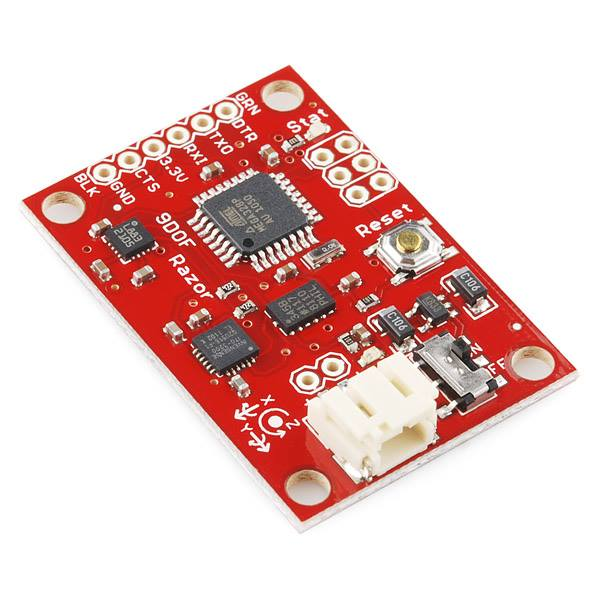
\includegraphics[scale=0.3]{imagenes/3-boomerang/IMU.jpg}
		\caption{9DOF Razor IMU de SparkFun.}
		\label{fig19}
		\end{center}
		\end{figure}
\newpage
	\subsubsection{Unidad de almacenamiento de datos}

	Para llevar un registro de los datos de los sensores se utiliza un módulo de tarjetas microSD, el cual utiliza el protocolo SPI (por sus siglas en inglés, Serial Peripheral Interface) y para cuya comunicación con la IMU se utiliza la libreria SD de Arduino.

		\begin{figure}[h]
		\begin{center}
		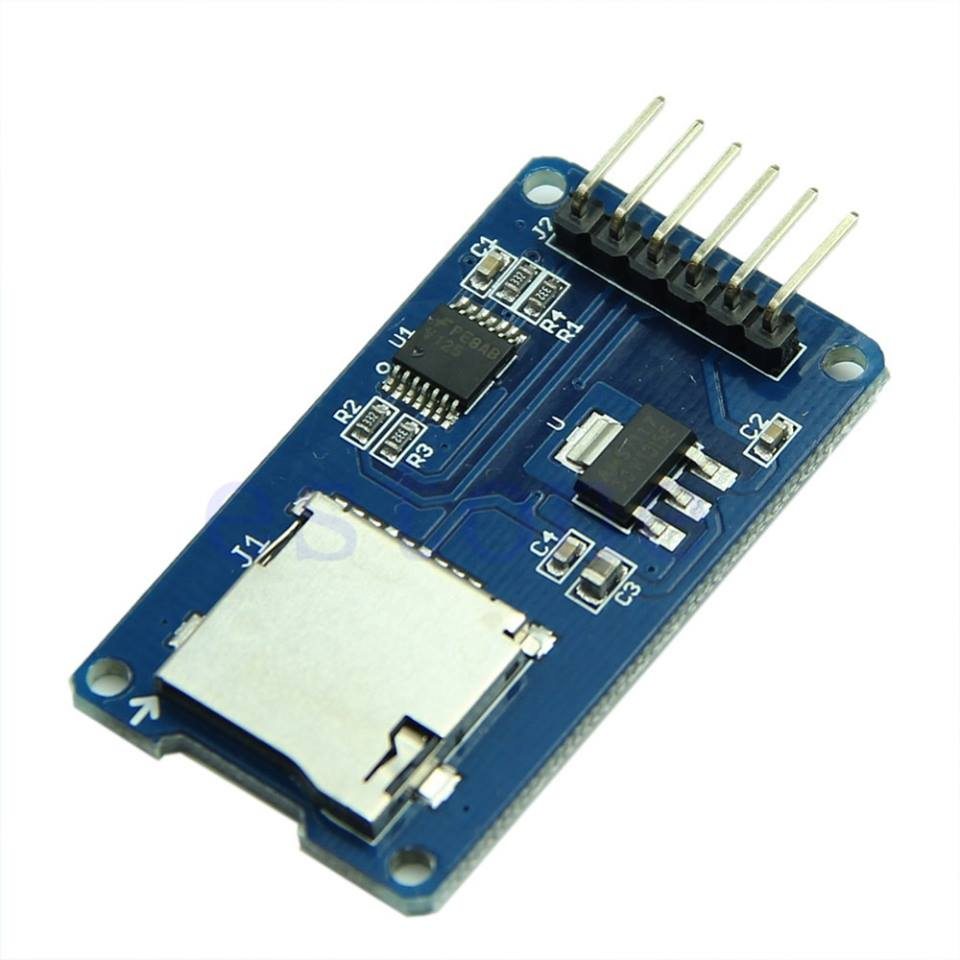
\includegraphics[scale=0.2]{imagenes/3-boomerang/SD.png}
		\caption{Módulo de tarjetas microSD de Arduino.}
		\label{fig20}
		\end{center}
		\end{figure}

	\subsection{Algoritmo de la matriz de cosenos directores (DCM)}

	Por medio del algoritmo de la matriz de cosenos directores (DCM por sus siglas en inglés, Direction Cosine Matrix) se puede obtener la orientación de una IMU en terminos de ángulos de Euler (roll, pitch, yaw en nuestro caso) considerando compensaciones en las mediciones de los sensores (obtenidas combinando acelerómetros y gyroscopios) que permiten minimizar el error de medición.

	Los giroscopios son usados como la principal fuente de información de la orientación. Se integra la ecuación cinemática no lineal que relaciona la raza de cambio en la orientación del objeto a su taza de rotación y su orientación presente.

	Se tiene en cuenta que errores numéricos en la integración pueden violar gradualmente la restricción de ortogonalidad de la DCM, por lo que se hacen ajustes regulares en los elementos de la matriz.

	Ya que se tienden a acumular errores numéricos del gyroscopio (drift y offset) en los elementos de la DCM, se usan vectores de referencia para detectarlos y un controlador PI entre los estos errores y las entradas del gyroscopio para disiparlos más rapido de lo que se acumulan.

	En nuestro caso se utiliza un magnetómetro para detectar errores en yaw y el acelerómetro para detectar pitch y roll.

	El diagrama siguiente muestra la secuencia de procesamiento de la información de los sensores. Para profundizar en el tema, consultese \cite{Premerlany}.

		\begin{figure}[h]
		\begin{center}
		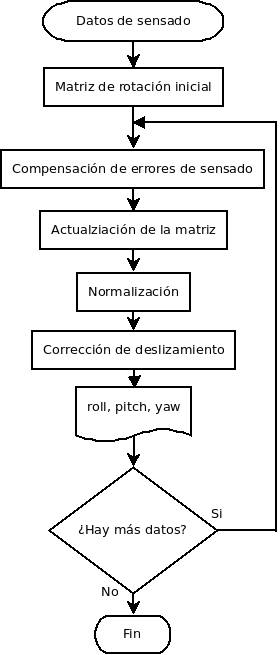
\includegraphics[scale=0.5]{imagenes/3-boomerang/DCM.jpg}
		\caption{Algoritmo DCM.}
		\label{fig24}
		\end{center}
		\end{figure}


	\subsection{Registrador de datos (Datalogger)}

Los datos de salida son almacenados en un archivo de extensión .CSV en una memoria microSD.

Se optó por implementar el algoritmo DCM en Matlab (fuera de línea), lo cual permitió deducir el periodo de muestreo a 10 ms.

Se notó que los tiempos entre adquisición de datos no se mantenían siempre en 10 ms, sino que se presentaban algunas veces periodos de 12 o incluso 20 ms. Por tanto se optó por almacenar también cada periodo de muestreo junto con los datos de los sensores en el archivo de salida.

	\subsection{Resultados del avance en la reconstrucción de la trayectoria de vuelo.}

	La trayectoria de vuelo de un boomerang se divide en orientación y posición en el espacio. La primera se obtiene utilizando el algoritmo de la matriz de cosenos directores, mientras que la segunda se obtiene al integrar dos veces los datos de aceleración del cuerpo respecto al sistema de referencia inercial.

	\subsubsection{Orientación en vuelo}

	La orientación del boomerang en vuelo es obtenida como resultado del algoritmo de la matriz de cosenos directores, el cual fue implementado en Matlab.

	La Fig. \ref{fig21} ilustra el cambio de orientación sufrido por el boomerang en instantes de tiempo $t = kT$, $k = {1, 2, 3, 4}$, de uno de los experimentos de recolección de datos inerciales realizados. Se puede notar el giro del boomerang respecto al eje Z que pasa por su centro de masa.

		\begin{figure}[h]
		\begin{center}
		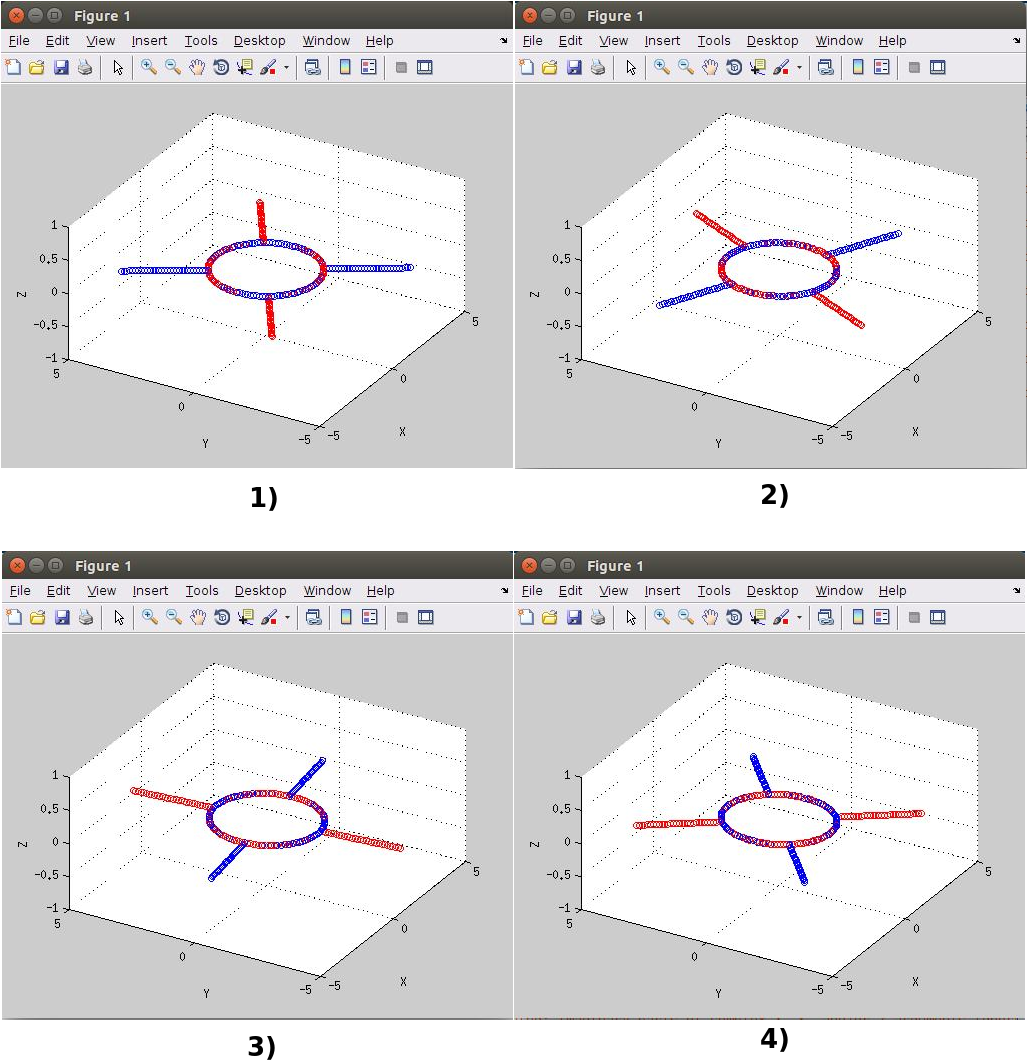
\includegraphics[scale=0.25]{imagenes/3-boomerang/orientacion_boomerang.png}
		\caption{Orientación del boomerang en vuelo en cuatro instantes de tiempo consecutivos.}
		\label{fig21}
		\end{center}
		\end{figure}

	\subsubsection{Trayectoria de vuelo}

	\subsubsection{Datos de aceleración respecto al sistema inercial}

	Para obtener información de velocidad y posición respecto al sistema de referencia inercial, es necesario primero obtener la aceleración física del sensor respecto a este sistema. Para esto, es importante primero entender exactamente qué es lo que mide un acelerómetro.

	Un vector de mediciones del acelerómetro ${a}_{m}$ puede ser modelado como:

	${ a }_{ m }={ a }_{ c }-{ R }^{ c }_{ I }\left( \begin{matrix} 0 \\ 0 \\ g \end{matrix} \right)$

	donde ${a}_{c}$ es la velocidad del sensor respecto al sistema fijo al cuerpo, g es la aceleración de la gravedad, y ${R}^{c}_{I}$ es la matriz de rotación del sistema de referencial inercial al sistema fijo al cuerpo. Este modelo asume que no hay errores en la medición.

	Para estimar la velocidad y posición,  necesitamos remover la componente de gravedad de la medición, por lo cual, despejando ${a}_{b}$ tenemos:

	${ a }_{ c }={ a }_{ m }+{ R }^{ c }_{ I }\left( \begin{matrix} 0 \\ 0 \\ g \end{matrix} \right)$

	Ahora la aceleración del cuerpo debe ser rotada de tal manera que sea representada en el sistema de referenciainercial, de tal manera que pueda ser integrada para obtener velocidad y posición. Esto nos lleva a:

	${ a }_{ I }={ R }^{ I }_{ c }{ a }_{ m }+\left( \begin{matrix} 0 \\ 0 \\ g \end{matrix} \right)$


	\subsubsection{Estimados de la velocidad y posición}

	Ya que se tienen las mediciones de la aceleración del sensor respecto al sistema inercial, pueden ser integrados para obtener estimados de la velocidad y posición.

	Se utilizó el metodo de integración numérica por trapecios de la siguiente manera:

	$v\left( k \right) =v\left( k-1 \right) +h\left( a\left( k \right) +a\left( k-1 \right) \right) /2$

	y de igual manera

	$p\left( k \right) =p\left( k-1 \right) +h\left( v\left( k \right) +v\left( k-1 \right) \right) /2$

	Los periodos de muestreo h utilizados en cada iteración de las dos integrales anteriores se obtienen del archivo .CSV del registrador de datos.

	\subsubsection{Resultados}

	Utilizando la teoría mencionada anteriormente se obtuvieron los siguientes resultados, los cuales no fueron satisfactorios debido a la gran diferencia entre los datos obtenidos y lo observado durante el experimento, que se asemejaba a los resultados de simulación.

	Recuerdese que el sistema de referencia inercial del sensor esta orientado de tal manera que el eje X apunta hacia el norte magnetico de la tierra, y el Z hacia abajo, por lo que los resultados mostrados en las Figs.  \ref{fig22} y \ref{fig23} nos dicen que la componente en Z de la posición incrementa en dirección ascendente (eje Z negativo), lo cual no es correcto.

		\begin{figure}[h]
		\begin{center}
		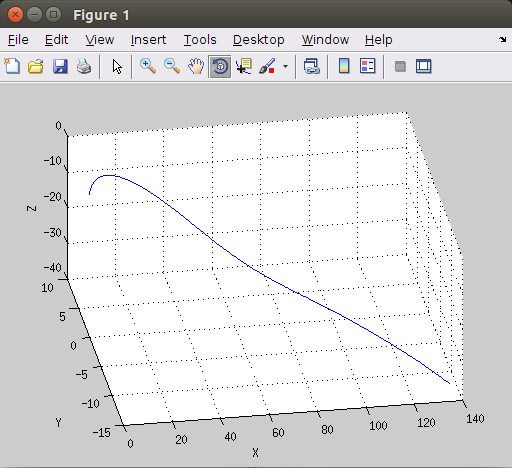
\includegraphics[scale=0.4]{imagenes/3-boomerang/tray_vue_1.jpg}
		\caption{Trayectoria de vuelo 1.}
		\label{fig22}
		\end{center}
		\end{figure}

		\begin{figure}[h]
		\begin{center}
		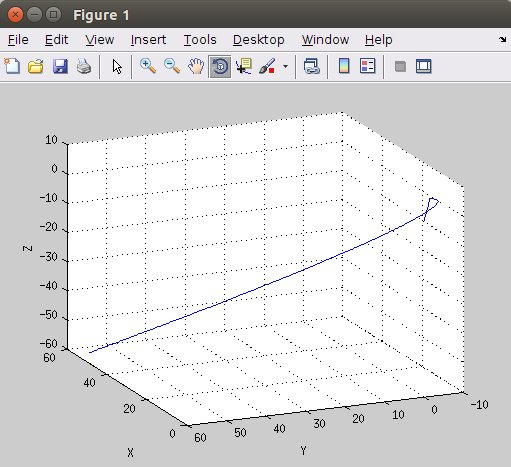
\includegraphics[scale=0.4]{imagenes/3-boomerang/tray_vue_2.jpg}
		\caption{Trayectoria de vuelo 2.}
		\label{fig23}
		\end{center}
		\end{figure}
\newpage
	\subsubsection{Posibles causas de error}

	Como se mencionó, los datos obtenidos no fueron los esperados, y entre las posibles causas están:

	\begin{enumerate}
	\item Mala interpretación de los datos obtenidos,
	\item Errores en la programación,
	\item Periodo de muestreo demasiado grande y datos con mucho ruido,
	\end{enumerate}

	los cuales son los puntos a revisar en trabajo futuro.
